\newproblem{09a}
{
	Triangles A and B are similar.\begin{center}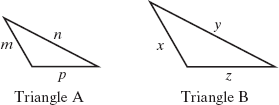
\includegraphics{fig100-09.png}\end{center} If $x=21$ in., $y=23$ in., and $m=19$ in., find the length of side $n$. Leave your answer as a fraction.
}
{
	\begin{tabular}{l r}
	$\dfrac{19}{21}=\dfrac{n}{23}$ or 
	$\dfrac{19}{n}=\dfrac{21}{23}$ or
	$\dfrac{21}{19}=\dfrac{23}{n}$ or 
	$\dfrac{n}{19}=\dfrac{23}{21}$ & 2 pts to here\\
	$n=\dfrac{437}{21}$ inches or $n= 20 \frac{17}{21}$ inches & 4 pts to here \\
	(3 pts for correct solution, but no units are given)
	\end{tabular}
}

\newproblem{09b}
{
	Triangles A and B are similar.\begin{center}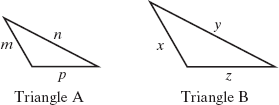
\includegraphics{fig100-09.png}\end{center} If $x=21$ in., $y=29$ in., and $m=17$ in., find the length of side $n$. Leave your answer as a fraction.
}
{
	\begin{tabular}{l r}
	$\dfrac{17}{21}=\dfrac{n}{29}$ or 
	$\dfrac{17}{n}=\dfrac{21}{29}$ or
	$\dfrac{21}{17}=\dfrac{29}{n}$ or 
	$\dfrac{n}{17}=\dfrac{29}{21}$ & 2 pts to here\\
	$n=\dfrac{493}{21}$ inches or $n= 23 \frac{10}{21}$ inches & 4 pts to here \\
	(3 pts for correct solution, but no units are given)
	\end{tabular}
}

\newproblem{09c}
{
	Triangles A and B are similar.\begin{center}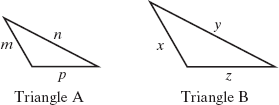
\includegraphics{fig100-09.png}\end{center} If $x=20$ in., $y=29$ in., and $m=13$ in., find the length of side $y$. Leave your answer as a fraction.
}
{
	\begin{tabular}{l r}
	$\dfrac{13}{20}=\dfrac{n}{29}$ or 
	$\dfrac{13}{n}=\dfrac{20}{29}$ or
	$\dfrac{20}{13}=\dfrac{29}{n}$ or 
	$\dfrac{n}{13}=\dfrac{20}{29}$ & 2 pts to here\\
	$n=\dfrac{377}{20}$ inches or $n= 18 \frac{17}{20}$ inches & 4 pts to here \\
	(3 pts for correct solution, but no units are given)
	\end{tabular}
}

\newproblem{09d}
{
	Triangles A and B are similar.\begin{center}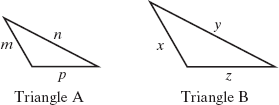
\includegraphics{fig100-09.png}\end{center} If $z=18$ in., $y=25$ in., and $n=9$ in., find the length of side $p$. Leave your answer as a fraction.
}
{
	\begin{tabular}{l r}
	$\dfrac{9}{25}=\dfrac{p}{18}$ or
	$\dfrac{9}{p}=\dfrac{25}{18}$ or 
	$\dfrac{25}{9}=\dfrac{18}{p}$ or 
	$\dfrac{p}{9}=\dfrac{18}{25}$ & 2 pts to here\\
	$p=\dfrac{162}{25}$ inches or $p= 6 \ffrac{12}{25}$ inches & 4 pts to here \\
	(3 pts for correct solution, but no units are given)
	\end{tabular}
}
